\section{First Problem Set}
\subsection{Introduction}
\textit{Give a brief description of your academic background and scientific interests. What is your major and what year are you in? If you work in a lab or research group, please give your supervisor's name and describe your project.}
\vspace{1em}

I received my bachelor's in Physics with a minor in Math from Western Kentucky University in Spring 2024. I'm now in my second year in both the Applied Physics and Scientific Computing PhD programs.
\vspace{1em}

My scientific interests revolve mostly around scientific computation rather than a single subfield of physics (though I really do enjoy plasma physics). I also have a strong interest in computational software and hardware and enjoy developing tools in my free time as well as working with enterprise server systems and software.
\vspace{1em}

I currently work with Alec Thomas in NERS on adding a photon kinetic framework to the OSIRIS particle-in-cell (PIC) code. In a very general sense, our group studies plasma-based wakefield accelerators, where a wake (analogous to waves/wakes generated by a duck moving through water) is driven by either a laser or a particle beam (the \textit{drive beam}) and used to accelerate a secondary beam (the \textit{witness beam}). 
\vspace{1em}

While the above describes the broader research area, our group is particularly interested in \textit{photon acceleration}. In conventional plasma-based particle accelerators, a particle or laser beam drives a wake in the plasma, and a trailing particle beam serves as the witness. In the case of photon acceleration, the witness particle beam is replaced with a laser or some other form of electromagnetic radiation. As this light interacts with the evolving plasma wake, it can experience frequency shifts, which we call photon acceleration (or deceleration). This process is of interest for applications such as the generation of tunable extreme-ultraviolet (XUV) radiation sources.
\vspace{1em}

From a computational perspective, photon acceleration can be difficult to model. Accurately resolving the electromagnetic fields requires time steps constrained by the Courant-\\Friedrichs–Lewy (CFL) condition. At the same time, the physical processes of interest occur over comparatively long length scales, which leads to simulations that must run for a large number of time steps. To address this, we're working on a photon kinetic model that instead treats radiation as an ensemble of quasi-particles evolving on longer timescales, which allows us to observe the photon acceleration phenomenon without explicitly resolving the electromagnetic field oscillations.

\subsection{Order of Accuracy in Forward and Central Differencing Schemes}
\textit{Let $f(x) = \sin{x}$ and take $x = \frac{\pi}{4}$, so that $f'(x) = f'(\frac{\pi}{4}) = \cos{\frac{\pi}{4}} = \frac{\sqrt{2}}{2} = 0.70710678$.}

\begin{enumerate}[label=(\alph*)]

  \item \textit{Take $h = 0.1, \,0.05, \,0.025, \,0.0125$ and present a table of the listed quantities. Indicate the limit of each column, as we did in class. We showed that $D_{+} f(x) = f'(x) + \frac{1}{2}f''(x)h + ...$, which implies that $D_{+} f(x)$ is 1st order accurate. Is your table consistent with this?}
      \vspace{1em}
      \newpage

    We are already given that $f'(\frac{\pi}{4}) = \frac{\sqrt{2}}{2} = 0.70710678$ as well as the values of $h$ to use, so we just need to evaluate $D_{+}f(x)$, which is just the forward-difference approximation:
    \begin{equation*}
      f'(x) = \frac{f(x+h)-f(x)}{h} = D_{+}f(x).
    \end{equation*}

    So for $h=0.1$, for example,
    \begin{equation*}
      D_{+}f(x) = \frac{\sin{\left(\frac{\pi}{4}+0.1\right)}-\sin{\left(\frac{\pi}{4}\right)}}{0.1} \approx 0.67060297. 
    \end{equation*}

    The table of all requested values is shown below as well as the limits of each column. I was unsure of the number of decimal digits to use, so I just used eight.

    \begin{table}[h!]
      \centering
      \begin{tabular}{|c|c|c|c|c|c|}
        \hline
        \rule{0pt}{3ex}$h$ & $D_{+}f(x)$ & $\abs{f'(x) - D_{+}f(x)}$ & $\frac{\abs{f'(x) - D_{+}f(x)}}{h}$ & $\frac{\abs{f'(x) - D_{+}f(x)}}{h^{2}}$ & $\frac{\abs{f'(x) - D_{+}f(x)}}{h^{3}}$ \\
        \hline
        0.1    & 0.67060297 & 0.03650381 & 0.36503810 & 3.6503810 & 36.503810 \\
        0.05   & 0.69813820 & 0.01796858 & 0.35937156 & 7.1874312 & 143.74862 \\
        0.025  & 0.69819475 & 0.00891203 & 0.35648116 & 14.259247 & 570.36986 \\
        0.0125 & 0.70266900 & 0.00443777 & 0.35502191 & 28.401753 & 2272.1403 \\
        \hline
        \multicolumn{1}{|c|}{\rule{0pt}{2.5ex}$\rightarrow 0$} & \multicolumn{1}{c|}{\rule{0pt}{2.5ex}$\rightarrow \sqrt{2}/2$} & \multicolumn{1}{c|}{\rule{0pt}{2.5ex}$\rightarrow 0$} & \multicolumn{1}{c|}{\rule{0pt}{2.5ex}$\rightarrow f''(\pi/4)/2$} & \multicolumn{1}{c|}{\rule{0pt}{2.5ex}$\rightarrow f''(\pi/4)/2h$} & \multicolumn{1}{c|}{\rule{0pt}{2.5ex}$\rightarrow f''(\pi/4)/2h^{2}$} \\
        \hline
      \end{tabular}
    \end{table}

    Although the last two columns are labeled using the same notation as in class,
    these quantities don't converge to finite limits as $h \to 0$. Rather, for each fixed $h$ the entries are finite, but as $h \to 0$ they grow without bound, diverging at rates proportional to $1/h$ and $1/h^2$, respectively. The expressions shown in the bottom row therefore describe the asymptotic growth of these columns rather than true limits.
    \vspace{1em}

    In the table, we can see that $\abs{f'(x)-D_{+}f(x)}/h$ approaches a finite limit, while the higher-order scaled errors diverge. This would imply that the forward-difference method is first-order accurate, which is consistent with what is mentioned in the problem statement.
    \vspace{1em}

  \item \textit{The central difference approximation for $f'(x)$ is $D_{0}f(x) = \frac{f(x+h)-f(x-h)}{2h}$. Show that $D_{0}f(x) = f'(x) + ch^{2} + ...$ for some constant $c$ which is independent of $h$.}
      \vspace{1em}

    To solve this problem, we just need to perform a Taylor expansion of both $f(x+h)$ and $f(x-h)$, then subtract the latter from the former and divide by $2h$. The standard form for the Taylor expansion is:
    \begin{equation*}
      f(x) = f(x_{0}) + f'(x_{0})(x-x_{0}) + \frac{f''(x_{0})}{2!}(x-x_{0})^{2} + ...,
    \end{equation*}

    but we'll call $x-x_{0} = h$, so that $x = x_{0}+h$, which will give us the correct form but with $x_0$ instead of $x$ (which we can just solve with a variable substitution), so we end up being able to write:
    \begin{equation*}
      f(x+h) = f(x) + f'(x)h + \frac{1}{2}f''(x)h^{2} + \frac{1}{6}f'''(x)h^{3} + ...
    \end{equation*}

    For the expansion of $f(x-h)$, we can just substitute all of our $h$'s for $-h$'s, such that we get:
    \begin{equation*}
      f(x-h) = f(x) - f'(x)h + \frac{1}{2}f''(x)h^{2} - \frac{1}{6}f'''(x)h^{3} + ...
    \end{equation*}

    Now we can subtract $f(x-h)$ from $f(x+h)$, which gives us:
    \begin{equation*}
      f(x+h) - f(x-h) = 2hf'(x) + \frac{2}{6}f'''(x)h^{3} + ...
    \end{equation*}

    Finally, divide by $2h$ to get the expression:
    \begin{equation*}
      D_{0}f(x) = \frac{f(x+h) - f(x-h)}{2h} = f'(x) + \frac{1}{6}f'''(x)h^{2} + ... =  \boxed{f'(x) + ch^{2} + ...}
    \end{equation*}

  \item \textit{Present a table for $D_{0}f(x)$ in the same format as part (a). What is the order of accuracy of $D_{0}f(x)$? For a given $h$, which approximation is more accurate, $D_{+}f(x)$ or $D_{0}f(x)$?}
      \vspace{1em}

    Before I get to the table, we just found in the previous part that 
    \begin{equation*}
      D_{0}f(x) = f'(x) + ch^{2} + ...,
    \end{equation*}

    where the $f'(x)$ term represents the actual value of the derivative and the $ch^{2}$ term represents the correction value (or error). Therefore, the order of accuracy for $D_{0}f(x)$ would be $\mathbf{O(h^{2})}$, whereas for the forward-difference approximation ($D_{+}f(x)$), the error is $O(h)$. So, for some given $h$, the \textbf{center-difference ($D_{0}f(x)$) approximation is more accurate}.
      \vspace{1em}

    Now, we present a table that's similar to the one before (again, I'm using eight decimal digits here):
    \begin{table}[h!]
      \centering
      \begin{tabular}{|c|c|c|c|c|c|}
        \hline
        \rule{0pt}{3ex}$h$ & $D_{0}f(x)$ & $\abs{f'(x) - D_{0}f(x)}$ & $\frac{\abs{f'(x) - D_{0}f(x)}}{h}$ & $\frac{\abs{f'(x) - D_{0}f(x)}}{h^{2}}$ & $\frac{\abs{f'(x) - D_{0}f(x)}}{h^{3}}$ \\
        \hline
        0.1    & 0.70592886 & 0.00117792   & 0.01177922 & 0.11779222 
               & 1.1779222 \\
        0.05   & 0.70681219 & 2.9459090$\times 10^{-4}$ & 0.00589182 & 0.11783640 
               & 2.3567280 \\
        0.025  & 0.70703313 & 7.3654655$\times 10^{-5}$ & 0.00294619 & 0.11784745 
               & 4.7138979 \\
        0.0125 & 0.70708837 & 1.8414097$\times 10^{-5}$  & 0.00147313 & 0.11785022 
               & 9.4280176 \\
        \hline
        \multicolumn{1}{|c|}{\rule{0pt}{2.5ex}$\rightarrow 0$} & \multicolumn{1}{c|}{\rule{0pt}{2.5ex}$\rightarrow \sqrt{2}/2$} & \multicolumn{1}{c|}{\rule{0pt}{2.5ex}$\rightarrow 0$} & \multicolumn{1}{c|}{\rule{0pt}{2.5ex}$\rightarrow hf'''(\pi/4)/6$} & \multicolumn{1}{c|}{\rule{0pt}{2.5ex}$\rightarrow f'''(\pi/4)/6$} & \multicolumn{1}{c|}{\rule{0pt}{2.5ex}$\rightarrow f'''(\pi/4)/6h$} \\
        \hline
      \end{tabular}
    \end{table}

    As in part (a), the last columns are shown using their asymptotic behavior: even if the values grow very large as $h \to 0$, each entry follows the pattern predicted by the leading term of the truncation error.

  \item \textit{Modify the Matlab code given in class to plot the error in $D_{+}f(x)$ and $D_{0}f(x)$ for step size $h = 1/2^{(j-1)}$ with $j = 1:65$. Use log scales for the error $\abs{f'(x)-Df(x)}$ and step size $h$. Plot both cases on the same graph. Explain the results.}
      \vspace{1em}

    I don't really use Matlab, so I replicated everything in Python and received the plot below.
    \begin{figure}[H]
      \centering
      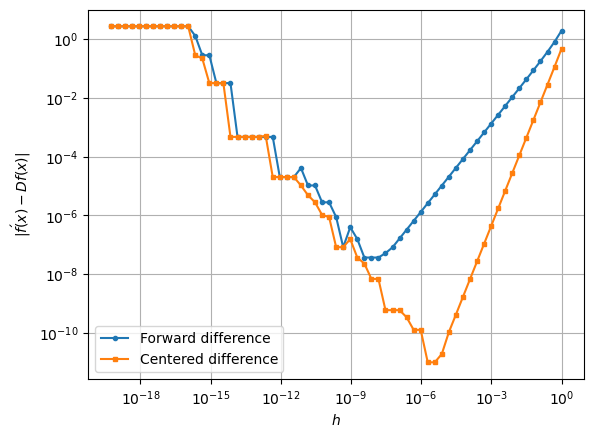
\includegraphics[width=0.65\textwidth]{figures/forvscent.png}
    \end{figure}
\end{enumerate}

From the log--log plot, we can see that the error in the forward-difference approximation decreases linearly with $h$, which corresponds to a slope of approximately $1$. This shows that, indeed, $D_{+}f(x)$ is first-order accurate. The error in the central-difference approximation decreases quadratically with $h$, which corresponds to a slope of approximately $2$. This shows that $D_{0}f(x)$ is second-order accurate. For sufficiently small step sizes, the central-difference method is therefore much more accurate than the forward-difference method.
\vspace{1em}

For very small values of $h$ (as on the left side of the above plot), the error no longer decreases and instead begins to increase. This is due to floating-point roundoff error. As $h \to 0$, the finite-difference formulas involve subtracting nearly equal numbers, which leads to a loss of significant digits. When these small differences are divided by $h$, roundoff errors are amplified, which eventually causes them to dominate the truncation error.

\subsection{Euler's Method for a Linear First-Order ODE}
\textit{Consider the problem $y' = ay+b$, $y(0) = y_{0}$, and let $u_{n}$ be the numerical solution at time $t=nh$ given by Euler's method. Find an expression for $u_{n}$, compute $\lim_{n\to\infty}{u_{n}}$, show that the limit satisfies the differential equation and initial condition.}
\vspace{1em}

This is a linear, first-order ODE, which can be solved directly. We can rewrite the differential equation as:
\begin{equation*}
  y' = ay+b \;\Rightarrow\; \dv{y}{t} = ay+b \;\Rightarrow\; \frac{\mathrm{d}y}{ay+b} = \mathrm{d}t.
\end{equation*}

Now integrate both sides:
\begin{equation*}
  \int \frac{\mathrm{d}y}{ay+b} = \int \mathrm{d}t \;\Rightarrow\; \frac{1}{a} \ln{(ay+b)} = t+C \;\Rightarrow\; y = Ke^{at} - \frac{b}{a},
\end{equation*}

where $K$ is a constant. If we apply the initial condition $y(0)=y_{0}$:
\begin{equation*}
    y_{0}=K-\frac{b}{a} \;\Rightarrow\; K=y_{0}+\frac{b}{a}.
\end{equation*}

So the \textbf{exact solution} is:
\begin{equation*}
    y(t) = \left(y_{0}+\frac{b}{a}\right)e^{at}-\frac{b}{a}.
\end{equation*}

To find an expression for $u_{n}$, we can start with the fact that $u_{n+1} = u_{n}+hf(u_{n})$, so:
\begin{equation*}
    u_{n+1} = u_{n} + h(au_{n}+b)=u_{n} + ahu_{n} + bh = (1+ah)u_{n} + bh,
\end{equation*}

and $u_{0} = y_{0}$. We can try to guess the pattern, and therefore $u_{n}$, by writing a few steps out:
\begin{align*}
    &u_{1} = u_{0}(1+ah) + bh \\
    &u_{2} = u_{1}(1+ah) + bh = (1+ah)^{2}u_{0}+bh[(1+ah)+1] \\
    &u_{3} = u_{2}(1+ah)+bh = (1+ah)^{3}u_{0}+bh \left[(1+ah)^{2}+(1+ah)+1\right] \\
    &\;\;\vdots \notag \\
    &u_{n} = (1+ah)^{n}u_{0}+bh \left[1+(1+ah)+(1+ah)^{2}+...+(1+ah)^{n-1}\right]
\end{align*}

This last term is a geometric sum, which for a finite series (as in our case), converges to
\begin{equation*}
  S_{n} = a_{1} \frac{(1-r^{n})}{(1-r)},
\end{equation*}

where $a_{1}$ is the first term in the series and $r$ is the common ratio. In this case, $a_{1}=1$ and $r=(1+ah)$, so:
\begin{align*}
  u_{n} &= (1+ah)^{n}u_{0} + bh \left[\frac{(1+ah)^{n}-1}{ah}\right] \\
        &= (1+ah)^{n}u_{0}  + \frac{b}{a}[(1+ah)^{n}-1] \\
        &= (1+ah)^{n}u_{0} + \frac{b}{a}(1+ah)^{n} - \frac{b}{a} \\
        &\boxed{= (1+ah)^{n} \left(u_{0}+\frac{b}{a}\right)-\frac{b}{a}.}
\end{align*}

For the limit of the above result to exist as $n\to\infty$, we require $\abs{1+ah} < 1$, which in particular requires that $a<0$ (and $h$ sufficiently small). If this is the case, then
\begin{equation*}
  \lim_{n\rightarrow\infty} u_{n} = -\frac{b}{a}.
\end{equation*}

To check if this satisfies the differential equation, we can plug in the solution $y = -\frac{b}{a}$, which yields:
\begin{equation*}
  \dv{y}{t} = a \left(-\frac{b}{a}\right) + b = 0,
\end{equation*}

which makes sense as $-\frac{b}{a}$ is a constant, so $\dv{t} \left(-\frac{b}{a}\right) = 0$. Also from the exact solution:
\begin{equation*}
    y(t) = \left(y_{0}+\frac{b}{a}\right)e^{at}-\frac{b}{a},
\end{equation*}

if $a<0$, then
\begin{equation*}
  \lim_{t\to\infty} e^{at} = 0,
\end{equation*}

so:
\begin{equation*}
  \lim_{t\to\infty} y(t) = -\frac{b}{a},
\end{equation*}

which matches the statement:
\begin{equation*}
    \lim_{n\to\infty} u_{n} = -\frac{b}{a}. 
\end{equation*}

\subsection{Convergence and Error Analysis of Euler's Method}
\textit{Consider the problem $y'=-y^{2}$, $y(0)=1$.}

\begin{enumerate}[label=(\alph*)]

    \item \textit{Find the exact solution $y(1)$.}
      \vspace{1em}

      To solve this, we can just use separation of variables. First, we rewrite the differential equation as:
      \begin{equation*}
        \dv{y}{t} = -y^{2} \;\Rightarrow\; -\frac{\mathrm{d}y}{y^{2}} = \mathrm{d}t.
      \end{equation*}

      After integrating both sides of the above:
      \begin{equation*}
        \frac{1}{y} + C_{1} = t + C_{2} \;\Rightarrow\; \frac{1}{y} = t+C \;\Rightarrow\; y = \frac{1}{t+C}.
      \end{equation*}

      Now, using the initial condition $y(0)=1$, we find that $C=1$ and therefore:
      \begin{equation*}
        y=\frac{1}{t+1}.
      \end{equation*}

      At $t=1$, then, $\boxed{y=\frac{1}{2}}$.

    \item \textit{Compute $y(1)$ by Euler's method with time step $h = 0.1, 0.05, 0.025, 0.0125$. Present a table (column 1: $h$, column 2: $u_{n}$, column 3: $u_{n}-y_{n}$, column 4: $(u_{n} - y_{n})/h$) and note that $t=nh=1$ and $y_{n}=y(1)$.}
      \vspace{1em}
    
      Using the differential equation we were given, we can rewrite Euler's method as:
      \begin{equation*}
        u_{n+1} = u_{n}+hf(u_{n}) \;\Rightarrow\; u_{n+1} = u_{n}-hu_{n}^2.
      \end{equation*}

      So, as an example calculation, for $h=0.1$ and therefore $n=10$,
      \begin{align*}
        &u_{1} = u_{0}-hu_{0}^2 = 1-(0.1)(1)^{2} = 1-0.1 = 0.9 \\
        &u_{2} = u_{1}-hu_{1}^{2} = 0.819 \\
        &u_{3} = u_{2}-hu_{2}^{2} \approx 0.752 \\
        &\;\;\vdots \notag \\
        &u_{10} = u_{9}-hu_{9}^{2} \approx 0.482.
      \end{align*}

      Following this process for each value of $h$ gives us the following table.
      \begin{table}[h!]
      \centering
      \begin{tabular}{|c|c|c|c|}
        \hline
        \rule{0pt}{3ex}$h$ & $u_{h}$ & $u_{h}-y_{h}$ & $(u_{h}-y_{h})/h$ \\
        \hline
        0.1    & 0.48171288 & -0.01828712 & -0.18287122 \\
        0.05   & 0.49110492 & -0.00889508 & -0.17790153 \\
        0.025  & 0.49561117 & -0.00438883 & -0.17555310 \\
        0.0125 & 0.49781987 & -0.00218013 & -0.17441005 \\ 
        \hline
      \end{tabular}
    \end{table}

    \item \textit{Find the principle error function $E(t)$ and evaluate $E(1)$. Compare with column 4.}
      \vspace{1em}

      From class, we know that $E' = f_{y}(y)E - \frac{1}{2}y''$, $E(0)=0$. We can find each of the individual components we need, then shove everything together. First, let's find $f_{y}(y)$:
      \begin{equation*}
        f_{y}(y) = \dv{y}f(y) = \dv{y} \left[-y^{2}\right] = -2y.
      \end{equation*}

      Next, we can find $y''$:
      \begin{equation*}
        y'' = \frac{\mathrm{d}^{2}}{\mathrm{d}t^{2}}[y(t)] = \frac{\mathrm{d}^{2}}{\mathrm{d}t^{2}} \left[\frac{1}{t+1}\right] = \dv{t} \left[-\frac{1}{(t+1)^{2}}\right] = \frac{2}{(t+1)^{3}}.
      \end{equation*}

      Finally, let's put everything together:
      \begin{equation*}
        E'(t) = -\frac{2}{t+1} E(t) - \frac{1}{2} \frac{2}{(t+1)^{3}} \;\Rightarrow\; E'(t) + \frac{2}{t+1}E(t) = -\frac{1}{(t+1)^{3}}.
      \end{equation*}

      We need to solve this differential equation to find $E(t)$. We can use an integrating factor:
      \begin{equation*}
        \mu = e^{\int \frac{2}{t+1} \mathrm{d}t} = e^{2\ln{\abs{t+1}}} = (t+1)^{2}.
      \end{equation*}

      Multiply both sides of the differential equation by the integrating factor:
      \begin{equation*}
        (t+1)^{2}E'(t) + 2(t+1)E(t) = -\frac{1}{t+1}.
      \end{equation*}

      Notice that the left-hand-side is just the time derivative of $E(t)(t+1)^{2}$, so we can write:
      \begin{equation*}
        \dv{t} \left[E(t)(t+1)^{2}\right] = -\frac{1}{t+1}.
      \end{equation*}

      If we integrate, we get that:
      \begin{equation*}
        E(t)(t+1)^{2} = -\ln{(t+1)} \;\Rightarrow\; \boxed{E(t) = -\frac{\ln{(t+1)}}{(t+1)^{2}}.}
      \end{equation*}

      Therefore, $E(1)$ is:
      \begin{equation*}
        E(1) = -\frac{\ln{(2)}}{(2)^{2}} \approx \boxed{-0.17329.}
      \end{equation*}

    \item \textit{Perform Richardson extrapolation on the values in column 2. Keep 8 decimal digits for the tables in (b) and (d).}

      In class, we found that for Euler's method:
      \begin{align*}
          A_{j0} &= y+O(h) \\
          A_{j1} &= 2A_{j0} - A_{j-1,0} = y+O(h^{2}) \\
          A_{j2} &= \frac{4A_{j1} - A_{j-1,1}}{3} = y+O(h^{3}) \\
          A_{j3} &= \frac{8A_{j2}-A_{j-1,2}}{7} = y+O(h^{4}).
      \end{align*}

      So, for the first column of our table ($A_{j0}$), we just need to use Euler's method (which we've already done in (b)). For all of the other columns, we can use previous values to calculate what we need:
      \begin{table}[h!]
      \centering
      \begin{tabular}{|c|c|c|c|c|c|}
        \hline
        \rule{0pt}{3ex}$j$ & $h$ & $A_{j0}$ & $A_{j1}$ & $A_{j2}$ & $A_{j3}$ \\
        \hline
        0 & 0.1    & 0.48171288 &  &  &  \\
        1 & 0.05   & 0.49110492 & 0.50049697 &  &  \\
        2 & 0.025  & 0.49561117 & 0.50011742 & 0.49999090 &  \\
        3 & 0.0125 & 0.49781987 & 0.50002857 & 0.49999895 & 0.50000010 \\
        \hline
      \end{tabular}
    \end{table}

\end{enumerate}

\subsection{Higher-Order Error Terms in Euler’s Method}
\textit{The numerical solution of $y' = f(y)$, $y(0)=y_{0}$ by Euler's method has an asymptotic expansion of the form $u_{n} = y_{n}+hE_{n}+h^{2}D_{n}+O(h^{3})$ as $h \rightarrow 0$, where $E_{n}=E(t_{n})$, $D_{n}=D(t_{n})$ for certain functions $E(t)$, $D(t)$.}

\begin{enumerate}[label=(\alph*)]

    \item \textit{The differential equation for $E(t)$ was derived in class; now find the equation for $D(t)$.}
      \vspace{1em}

      We are given that the numerical solution produced by Euler's method has the asymptotic expansion:
      \begin{equation*}
          u_n = y_n + hE_n + h^2 D_n + O(h^3), \quad \text{as } h \to 0.
      \end{equation*}

      We can define the error as:
      \begin{equation*}
          e_{n} = u_{n} - (y_{n} + hE_{n} + h^{2}D_{n}),
      \end{equation*}

      such that $e_{n}=O(h^{3})$. 

      Now, we can plug this into Euler's method (which states that $u_{n+1} = u_n + h f(u_n)$). The left-hand-side becomes
      \begin{equation*}
          u_{n+1} = y_{n+1} + hE_{n+1} + h^{2}D_{n+1} + e_{n+1}.
      \end{equation*}

      The right-hand-side becomes
      \begin{equation*}
          u_{n} + hf(u_{n}) = y_{n} + hE_{n} + h^{2}D_{n} + e_{n} + hf(y_{n}+hE_{n}+h^{2}D_{n}+e_{n}).
      \end{equation*}

      Next, we need to Taylor expand $f(u_{n})$:
      \begin{align*}
        f(u_{n}) &= f(y_{n}+hE_{n}+h^{2}D_{n}+e_{n}) \\
                 &= f(y_{n}) + f'(y_{n})(hE_{n}+h^{2}D_{n}+e_{n}) + \frac{1}{2}f''(y_{n})(hE_{n}+h^{2}D_{n}+e_{n})^{2} + O(h^{3}).
      \end{align*}

      Multiplying by $h$ and keeping terms through $O(h^3)$,
      \begin{align*}
        hf(u_{n}) &= hf(y_{n}) + hf'(y_{n})(hE_{n}+h^{2}D_{n}+e_{n}) + \frac{1}{2}hf''(y_{n})(hE_{n}+h^{2}D_{n}+e_{n})^{2} + O(h^{4}) \\
                  &= hf(y_{n}) + h^{2}E_{n}f'(y_{n}) + h^{3}\left[\frac{1}{2}E_{n}^{2}f''(y_{n}) + D_{n}f'(y_{n})\right] + O(h^{4}).
      \end{align*}

      Note that the second line in the result above is after many simplifications that I didn't feel the need to re-type from my scratch paper. If we also expand the exact solution, we see that it satisfies
      \begin{equation*}
          y_{n+1} = y_{n} + y_{n}'h+\frac{1}{2}y_{n}''h^{2} + \frac{1}{6} y_{n}'''h^{3}+O(h^{4}),
      \end{equation*}

      with $y_n' = f(y_n)$.
      \vspace{1em}

      Substituting all expansions into Euler’s method and cancelling common terms yields
      \begin{align*}
        hE_{n+1} + h^{2}D_{n+1} &= hE_{n} + h^{2}D_{n} + h^{2}f'(y_{n})E_{n} + h^{3} \left[f'(y_{n})D_{n}+\frac{1}{2}f''(y_{n})E_{n}^{2}\right] \\
        &\quad - \frac12 h^2 y_n'' - \frac16 h^3 y_n''' + O(h^4).
      \end{align*}

      Since $e_n, e_{n+1} = O(h^3)$, their contributions are absorbed into the higher-order remainder and don't affect the equations at order $h^2$.
      \vspace{1em}

      Dividing by $h$ and grouping like powers gives
      \begin{align*}
        E_{n+1} - E_n &= h\left[f'(y_n)E_n - \frac12 y_n''\right] + O(h^2), \\
        D_{n+1} - D_n &= h\left[f'(y_n)D_n + \frac12 f''(y_n)E_n^2 - \frac16 y_n'''\right] + O(h^2).
      \end{align*}

      Taking the limit as $h \to 0$, we find the differential equations
      \begin{align*}
        E'(t) &= f'(y(t))E(t) - \frac12 y''(t), \\
        \Aboxed{D'(t) &= f'(y(t))D(t) + \frac12 f''(y(t))E(t)^2 - \frac16 y'''(t).}
      \end{align*}

    \item \textit{Consider the problem $y'=y$, $y_{0}=1$. In class, we showed that $E(t)=-\frac{1}{2}te^{t}$. Find $D(t)$.}
      \vspace{1em}

      We just found that the second-order error coefficient satisfies
      \begin{equation*}
          D'(t) = f'(y(t))D(t) + \frac{1}{2} f''(y(t))E(t)^{2} - \frac{1}{6}y'''(t).
      \end{equation*}

      For this problem, $f(y)=y$, so $f'(y)=1$ and $f''(y)=0$. The exact solution of the given differential equation is
      \begin{equation*}
        \dv{y}{t} = y \;\Rightarrow\; \frac{\mathrm{d}y}{y} = \mathrm{d}t \;\Rightarrow\; \ln{(y)} = t \;\Rightarrow\; y(t) = e^{t}.
      \end{equation*}

      Therefore, $y'''(t) = e^{t}$. Substituting into the equation for $D'(t)$ gives
      \begin{equation*}
          D'(t) = D(t)-\frac{1}{6}e^{t},
      \end{equation*}

      with $D(0)=0$, since the asymptotic expansion
      \begin{equation*}
          u_n = y(t_n) + h E(t_n) + h^2 D(t_n) + O(h^3)
      \end{equation*}

      must agree with the exact initial value at $t=0$, which implies that all higher-order error coefficients go away at $t=0$.
      \vspace{1em}

      We can solve this linear ODE using an integrating factor. Writing the equation as
      \begin{equation*}
          D'(t) - D(t) = -\frac{1}{6}e^{t},
      \end{equation*}

      the integrating factor is $\mu(t) = e^{-t}$. Multiplying both sides by $\mu(t)$:
      \begin{equation*}
        D'(t)e^{-t} - D(t)e^{-t} = -\frac{1}{6}.
      \end{equation*}

      The left-hand-side of this equation is the derivative of $D(t)e^{-t}$, so
      \begin{equation*}
        \dv{t}\left[D(t)e^{-t}\right] = -\frac{1}{6}.
      \end{equation*}

      Integrating and using $D(0)=0$, we get that:
      \begin{equation*}
        D(t)e^{-t} = -\frac{1}{6}t \;\Rightarrow\; \boxed{D(t) = -\frac{1}{6}te^{t}.}
      \end{equation*}

    \item \textit{Compute $y(1)$ by Euler's method with time step $h=0.1, 0.05, 0.025, 0.0125$. Present a table (column 1: $h$, column 2: $u_{n}$, column 3: $u_{n}-y_{n}$, column 4: $(u_{n} - y_{n})/h$, column 5: $u_{n} - (y_{n}+hE_{n})$, column 6: $(u_{n} - (y_{n}+hE_{n}))/h^2$) and evaluate $E(1)$ and $D(1)$; are they consistent with the table?}
      \vspace{1em}

      We know that Euler's method states that $u_{n+1} = u_{n}+hf(u_{n})$, which in this case ($y'=y$), just means that $u_{n+1} = u_{n}+hu_{n}=(1+h)u_{n}$. If we evaluate a few steps:
      \begin{align*}
          &u_{1} = (1+h)u_{0}=(1+h) \\
          &u_{2} = (1+h)u_{1} = (1+h)^{2} \\
          &u_{3} = (1+h)u_{2} = (1+h)^{3} \\
          &\;\;\vdots \notag \\
          &u_{n} = (1+h)^{n}
      \end{align*}

      After computing all of the necessary values, we get a table that ends up looking like (again with eight decimal digits):
      \begin{table}[h!]
      \centering
      \begin{tabular}{|c|c|c|c|c|c|}
        \hline
        \rule{0pt}{3ex}$h$ & $u_{n}$ & $u_{n}-y_{n}$ & $(u_{n}-y_{n})/h$ & $u_{n} - (y_{n}+hE_{n})$ & $(u_{n} - (y_{n}+hE_{n}))/h^2$ \\
        \hline
        0.1    & 2.5937425 & -0.12453937 & -1.2453937 & 0.01137472
               & 1.1374723 \\
        0.05   & 2.6532977 & -0.06498412 & -1.2996825 & 0.00297292
               & 1.1891690 \\
        0.025  & 2.6850638 & -0.03321799 & -1.3287196 & 7.6053279$\times 10^{-4}$
               & 1.2168525 \\
        0.0125 & 2.7014849 & -0.01679689 & -1.3437510 & 1.9237372$\times 10^{-4}$
               & 1.2311918 \\
        \hline
      \end{tabular}
    \end{table}

    Note that the exact solution at $y(1)$ is $e \approx 2.71828$, which is what column two is approaching. Also note that $E(1)$ is:
    \begin{equation*}
      E(1) = -\frac{1}{2}(1)e^{(1)} = \boxed{-\frac{1}{2}e \approx -1.35914,}
    \end{equation*}

    and $D(1)$ is:
    \begin{equation*}
      D(1) = -\frac{1}{6}(1)e^{(1)} = \boxed{-\frac{1}{6}e \approx -0.45305.}
    \end{equation*}

    Euler's method is first–order accurate, so the leading global error term is $O(h)$. As a result, column four correctly approaches $E(1)$, while the higher–order quantity in column six doesn't reliably converge to $D(1)$.

\end{enumerate}
